Dans le but de coordonnées les interactions entre ses partenaires, \textsf{EVOLLIS} 
échange avec ceux-ci des flux d'informations qui constituent de gros volumes de 
données hétérogènes. Aussi \textsf{EVOLLIS} propose l'offre \textsf{uZ'it} via une 
vignette image apparaissant sur la fiche produit du distributeur. La plateforme
d'Evollis fera donc l'objet d'un accès concourant aux données et d'un fort trafic.
Le but principale d'\textsf{EVOLLIS} est de pouvoir répondre efficacement aux 
différentes requêtes de génération de vignettes produits.
\begin {figure}[H]
       \centering
        %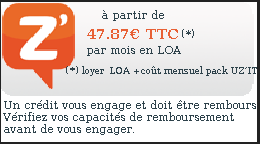
\includegraphics[width=12cm,height=4cm]{\DIR/img/vignette.PNG}
        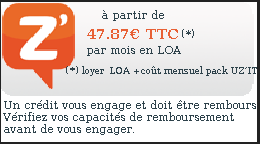
\includegraphics[scale=1]{\DIR/img/vignette.PNG}		
        \caption{Exemple de vignette produit avec un loyer de 38.43 €}
	\label{sqoop}
  \end {figure}    
\noindent
\textsf{EVOLLIS} génère les vignettes à la volée. Le loyer est calculé à partir de 
données stockées en base. À chaque génération de vignette correspondent plusieurs 
accès à la base de données et éventuellement un recalcul du loyer si les données 
transmises par le distributeur ne correspondent pas à celles présentes en base.
La génération des vignettes peut beaucoup impacter sur le temps de réponse de 
la plateforme. Pour ce faire, \textsf{EVOLLIS} met en place un système de cache
pour éviter de régénérer les vignettes produits dont les données n'ont pas changé en base. 
Le mécanisme est illustré par le schéma ci-dessous.
\begin {figure}[H]
       \centering
        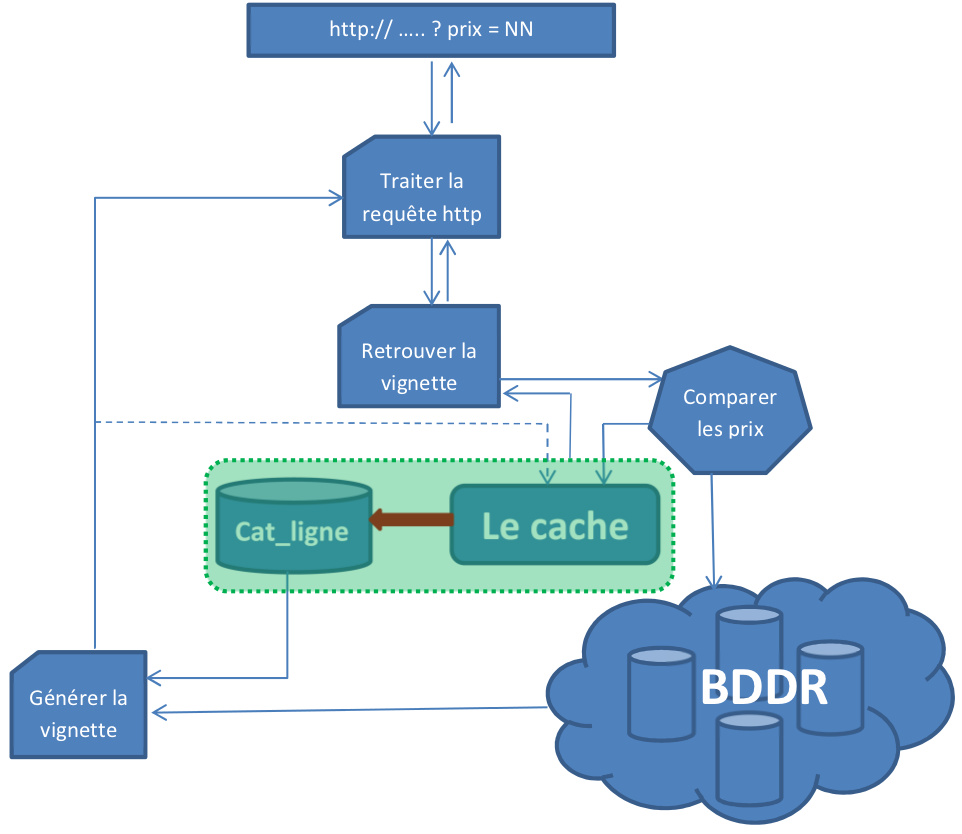
\includegraphics[scale=0.3]{\DIR/img/contexte.png}	
        \caption{Mécanisme de génération d'une vignette produit}
	\label{sqoop}
  \end {figure}    
\noindent
Avec l'apparition du \textsf{web 2.0} dans les années $2000$, le nombre d'internautes 
a considérablement augmenté. Les sites de commerce rencontrent deux problèmes majeurs
qui sont d'une part la taille et l'hétérogénéité des données stockées en base et d'autre part
le temps de réponse. Dans le cadre du stage \textsf{EVOLLIS} est intéressé par une solution
qui optimiserait la gestion des vignettes. À l'appel du \textsf{Web Service} de génération
de vignette, les deux entités table en base « \textsf{cat\_ligne} » et cache entrent en jeu 
conformément au mécanisme de génération de vignette défini plus haut. Les solutions non 
relationnelles de gestions des données connues sous la dénomination « \textsf{NoSQL} » 
proposent de nouvelles alternatives d'organisations physiques des données. L'idée ici du stage 
étant de voir comment tenir compte de celles-ci afin de fusionner la table en base 
« \textsf{cat\_ligne} » et le cache en une seule entité pour meilleure gestion des vignettes comme
l'illustre le schéma ci-dessous. 
\begin {figure}[H]
       \centering
        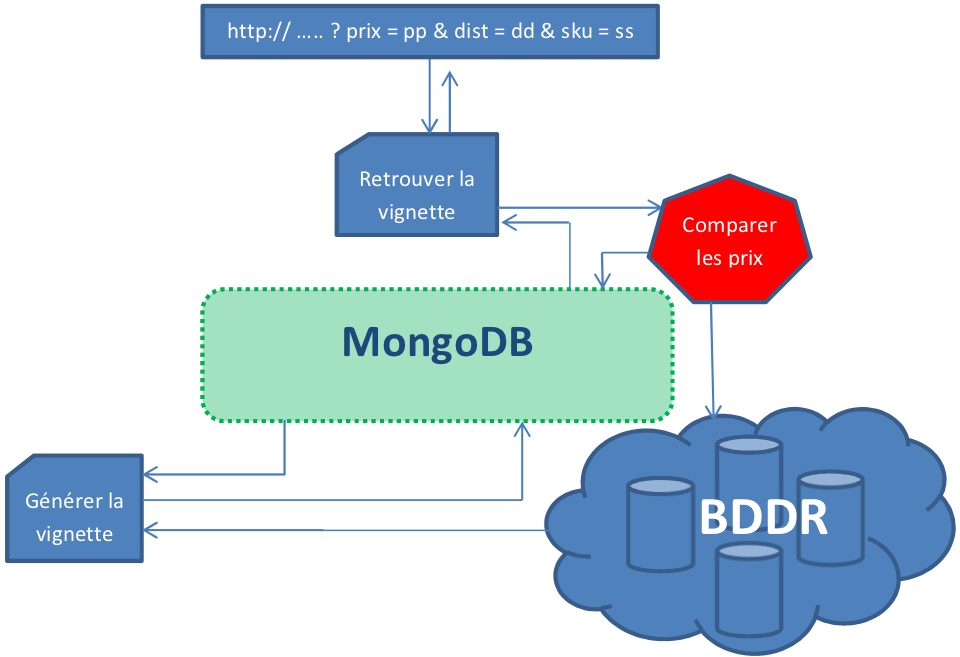
\includegraphics[scale=0.3]{\DIR/img/contexte1.png}	
        \caption{Mécanisme de génération d'une vignette produit}
	\label{sqoop}
  \end {figure}    

\subsection{Étude du gain de la fusion}
Nous allons dans un premier temps 

%%Evollis sera plus tenté par la solution NoSQL qui gère efficacement le stockage des vignettes.
%%Dans un premier temps dans le cadre du stage, il s'agit de faire un état de l'art, de faire
%%des tests de charges et d'en retenir la solution qui  

%% Sur un site de vente en ligne partenaire d'EVOLLIS, si un client forme un panier et décide de le payer, par le biais d'une vignette EVOLLIS sur laquelle le client pourra ensuite cliquer pour profiter de l'offre \textsf{lizéa}. Le calcul des tarifs de l'offre est effectué  à partir des identifiants des produits dans le panier du client et    


%% Evollis se place entre plusieurs partenaires commerciaux afin de 
%% coordonner leurs interactions.


%% Les cash sont volatiles, il faut à chaque les réconstitués. Les cash
%% fonctionnent en clé-valeur comme la plupart des gestionnaires NoSQL.
%% EVOLLIS veut en lieu et place du système de cash mettre un système de
%% hashage persistant apportant les mêmes performances qu'un accès cash.
%% Le Benefice étant que cette fois on a un systant persistant. À priori

%% le s'est pausé sur MongoDB. En arrière plan MongoDB reste une base
%% clef/valeur où la valeur est un document JSON complet. Cependant,
%% contrairement aux bases purement clef/valeur, il est possible de
%% requêter sur n’importe quel élément du document ou sous document.
